\documentclass[simplex.tex]{subfiles}
% NO NEED TO INPUT PREAMBLES HERE
% packages are inherited from simplex.tex; you can compile this on its own

\onlyinsubfile{
\title{NeuroData SIMPLEX Report: Subfile}
}

\begin{document}
\onlyinsubfile{
\maketitle
\thispagestyle{empty}

The following report documents the progress made by the labs of Randal~Burns and Joshua~T.~Vogelstein at Johns Hopkins University towards goals set by the DARPA SIMPLEX grant.

%%%% Table of Contents
\tableofcontents

%%%% Publications
\bibliographystyle{IEEEtran}
\begin{spacing}{0.5}
\section*{Publications, Presentations, and Talks}
\vspace{-20pt}
\nocite{*}
{\footnotesize	\bibliography{simplex}}
\end{spacing}
%%%% End Publications
}

\subsection{Graph Explorer}

We are building graph explorer as a first step towards modifying MEDA for graphs.  
The graph explorer now has new ability to view statistics conditional on the attributes in the graph, see figure~\ref{fig:graphExplorer}. The conditional distributions illustrate
the similarity and distinction among the different vertices in the
network data. Difference among these distributions are potentially
linked to their different functions in physiology.
Graph explorer is available at \url{http://shiny.neurodata.io/lduan/graphX/}.


\begin{figure}[h!]
\begin{cframed}
\centering
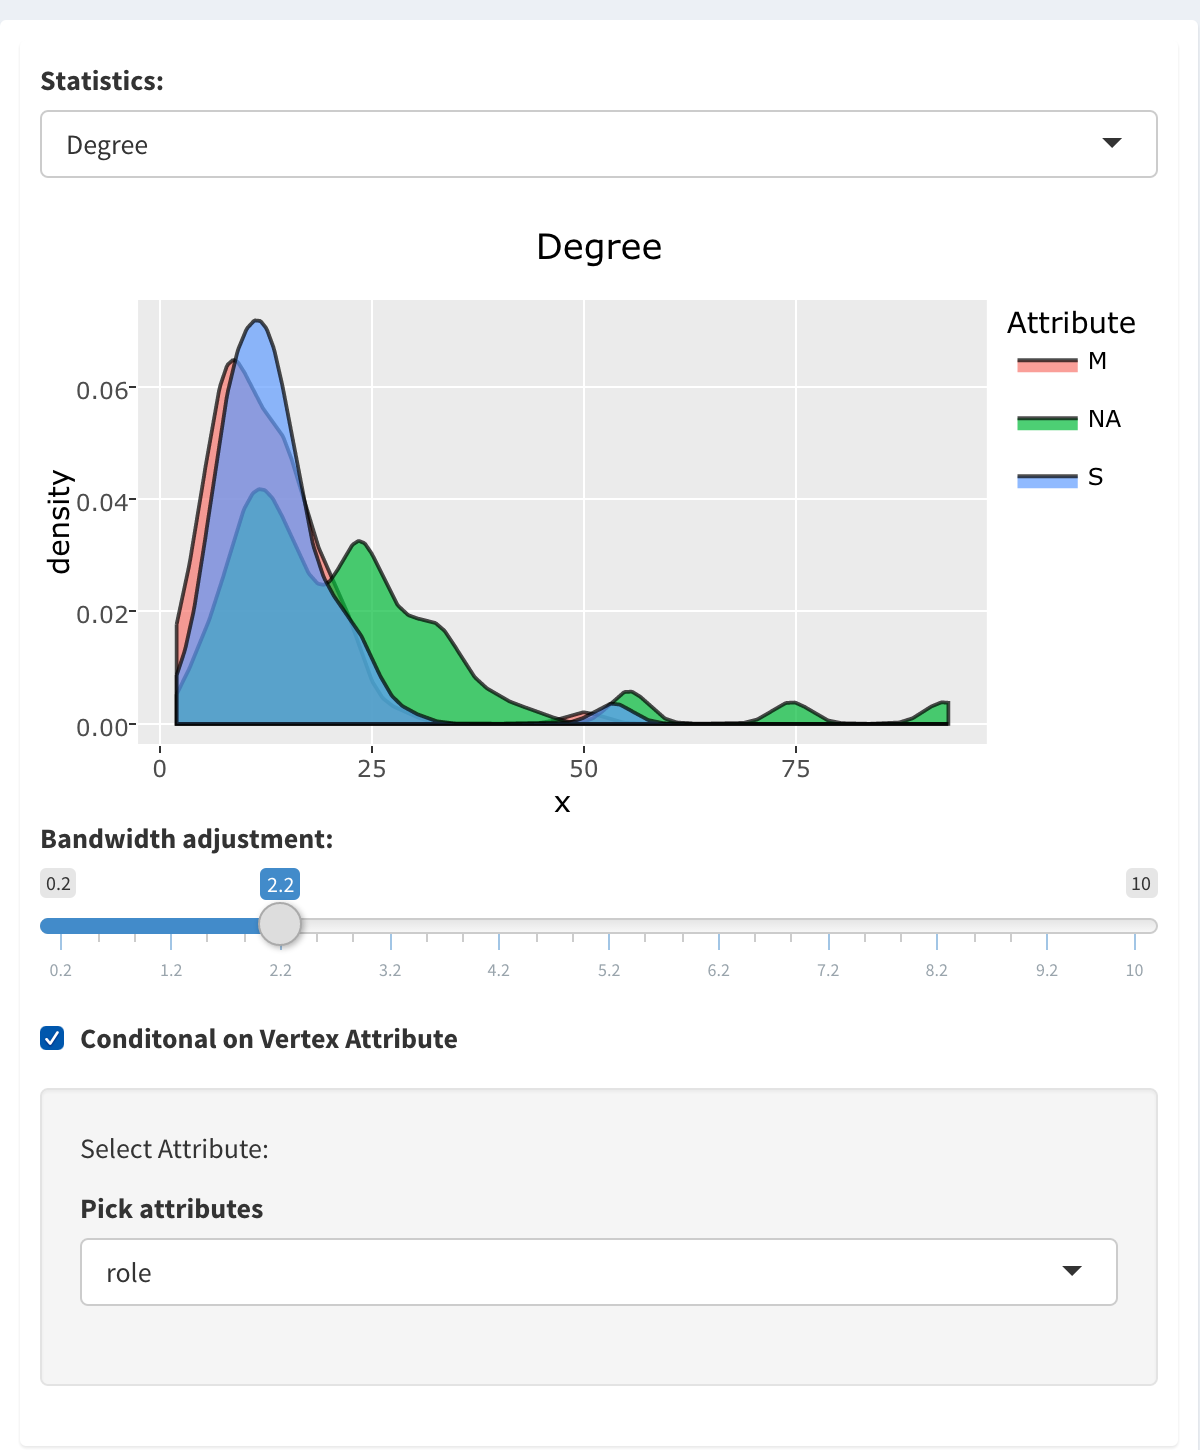
\includegraphics[width=0.5\textwidth]{../../figs/graph-explorer.png}
\caption{Graph Explorer interactivity example.}
\label{fig:graphExplorer}
\end{cframed}
\end{figure}
\end{document}
